%================================================================
\section{Results and Discussion}\label{sec:Results}
%================================================================

%----------------------------------------------------------------
\subsection{Non-Interacting}\label{sec:project results}
%----------------------------------------------------------------

\autoref{fig:train_iter_lr_batch1000} and \autoref{fig:train_iter_lr_batch5000} We vary the number of training iterations and the the learning rate, $\eta$. The training, or update of parameters, are done in batches of 5000 iterations, meaning that the x-axis tick labels correspond to the number of updates. 

Each point is the average of 8 Markov chains, each with expectation value of the energy, $\langle E \rangle$, the variance $\mathrm{Var}(E)$ and sampling error, $\sigma_b$, found via the blocking method, estimated from $2^{18}$ samples. The scales of the proposal distributions, $\sigma_p$, are set to $\sigma_p=3.0$ and $\sigma_p=1.3$ for the RWM and LMH algorithms, respectively, which give acceptance rates of $\sim 30\%$ and $\sim60\%$, respectively. 

System: 1 particle in 1 dimension, 2 hidden neurons, with the variance in the Gaussian layer set as $\sigma_\mathrm{RBM}^2=1.0$

\begin{figure}[!htb]
\begin{center}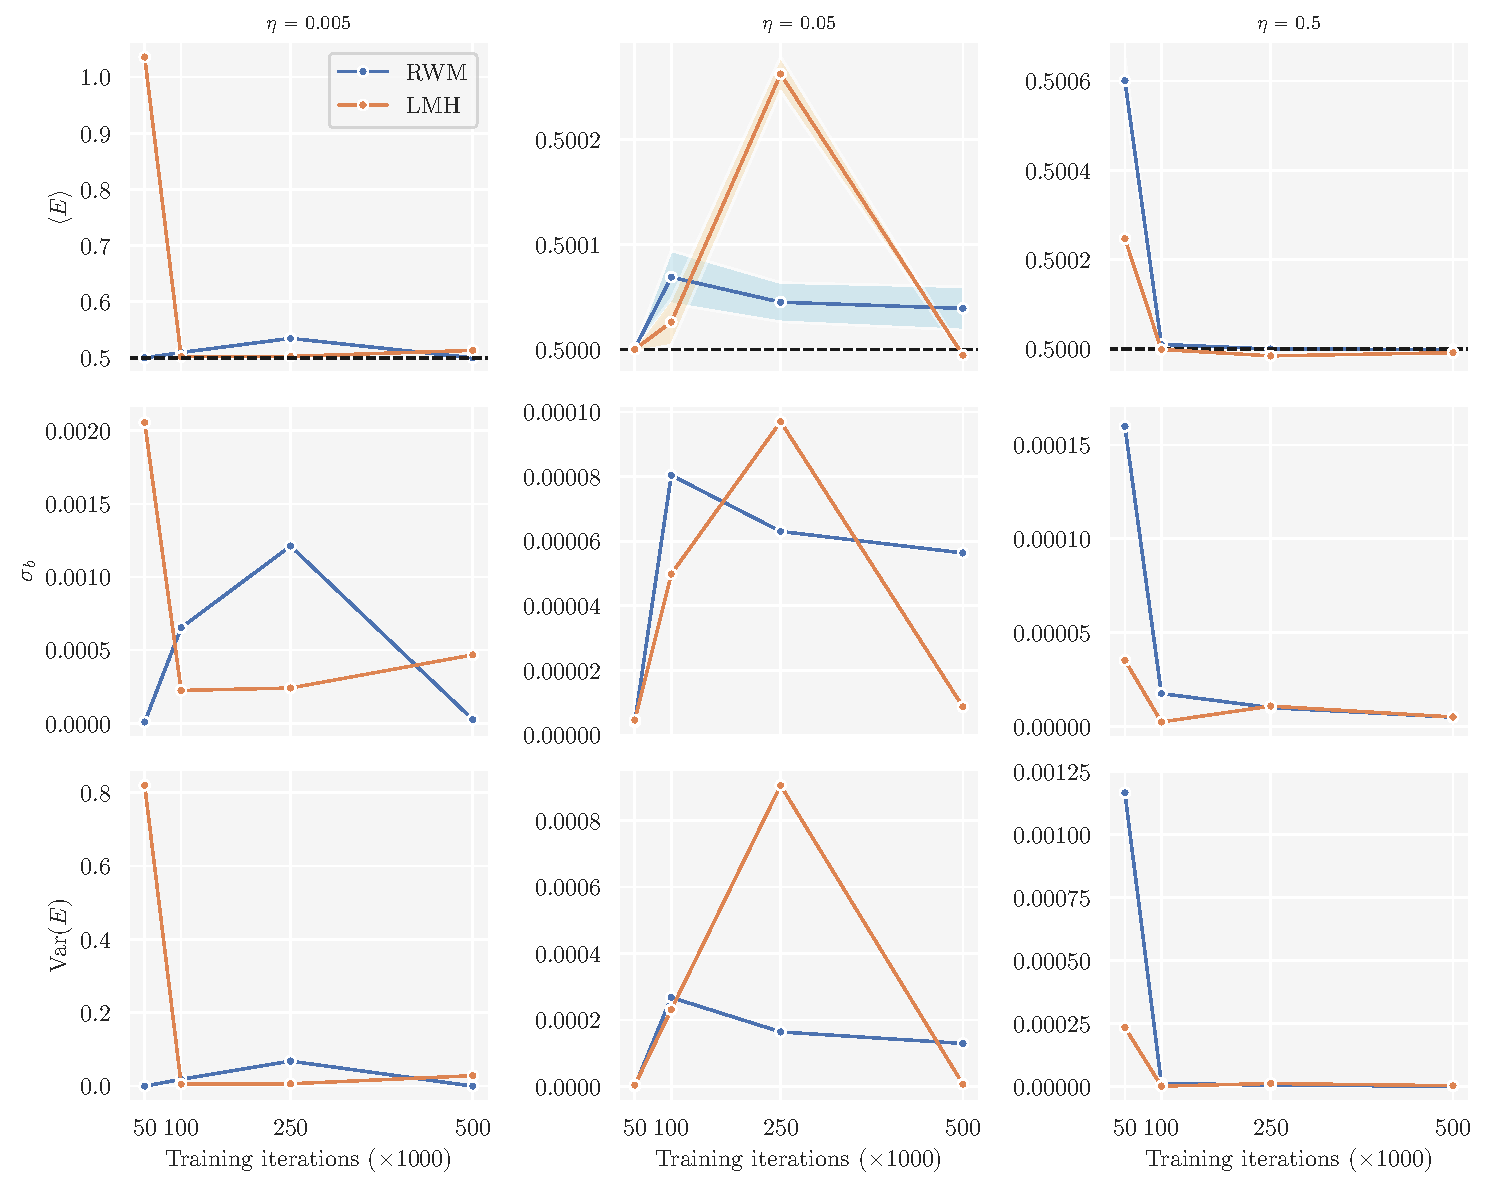
\includegraphics[width=\textwidth]{latex/figures/training_cycles_lr_batch1000.pdf}
\end{center}
\caption{c}
\label{fig:train_iter_lr_batch1000}
\end{figure}

\begin{figure}[!htb]
\begin{center}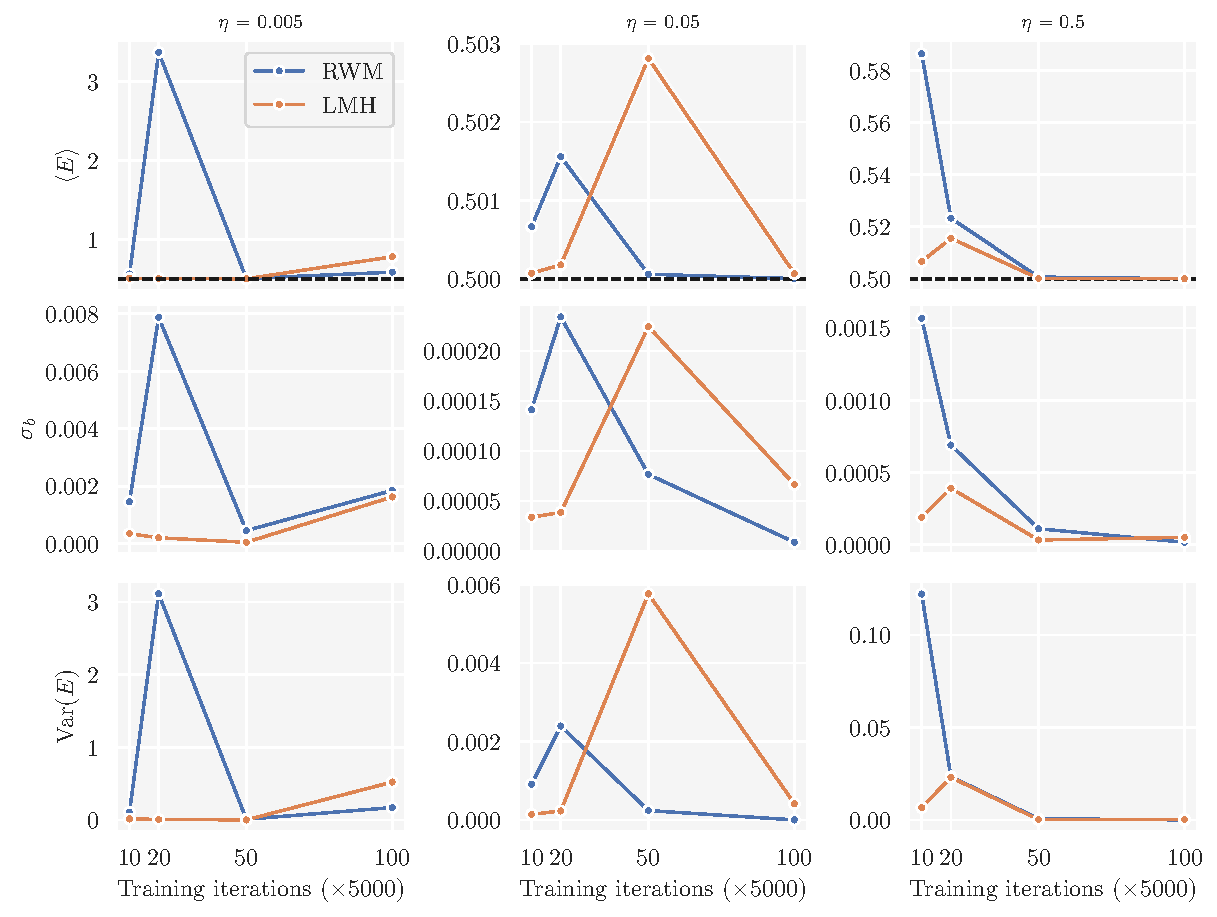
\includegraphics[width=\textwidth]{latex/figures/training_cycles_lr.pdf}
\end{center}
\caption{c}
\label{fig:train_iter_lr_batch5000}
\end{figure}

